\chapter{Arrays, Plotting and Chaos}

\section{Introduction}

This lab will introduce a fundamental element of scientific python,
the numpy array, and use them to produce plots.  We will also consider
the non-linear logistics map and examine bifurcation in the approach
to chaos.

If you can complete all of the plots in Section~\ref{sec:logmap}
including the optional plot and {\em without any instructor help} then
you may omit the plots from the preceding sections.

\section{Preparation}
\label{sec:arraysprep}

This lab will rely on the material from Sections 1.4.1 to 1.4.2 and
1.5.1 to 1.5.2 of the Scientific Python Lecture notes.  This is the
first lab that relies on inline plotting, so make sure you are
starting your notebook with the ``line magic'':
\begin{python}
  %pylab inline
\end{python}
This will load the numpy library as np, the matplotlib.pyplot library
as plt, and setup the matplotlib backend to imbed plots in your
notebook.

A Numpy array is a grid of values.  Unlike Python lists, the elements
of a numpy array all have the same data type, which makes them much
more computionally efficient.  Choices for the data type include the
built-in python integer, float, and bool types.  The numpy library
provides a wide range of analysis tools that are mostly centered on
the numpy array type.

Numpy arrays can be constructed easily from a Python list:
\begin{python}
a = np.array([1.3,7.2,4.1,0.0])
b = np.array([[1,2],[3,4]])
print(a)
print(b)
print(np.shape(a))
print(np.shape(b))
\end{python}
This is conveninent when you have specific values you want to define by hand.  Another possibility is to construct the numpy array by calling a function designed specifically for the purpose:
\begin{python}
a = np.linspace(0,1,11)
print(a)
b = np.arange(0,5,1)
print(b)
\end{python}
Both \pyth{linspace} and \pyth{arange} allow you to specify the range
of values you want, but with \pyth{linspace} you specify the number of
points you want whereas with \pyth{arange} you specify the step size.

One of the great joys of using numpy arrays comes from the fact that
most operators are applied elementwise automatically, without the need
to explictly write a for loop:
\begin{python}
a = np.arange(0,5,1)
b = 10
print(a)
print(b)
print(a+b)
\end{python}
Notice how the value of $b$ (10) is added to {\em every element} of
$a$, without the need to explicitly loop over every element.  Try
modify the example code to multiply every element of $a$ by $b$. Then
try raising each element of $a$ to the power of 2. \\

\plot Use numpy arange and elementwise operations to implement a
function \pyth{def powers(a, n)} which returns a numpy array
containing the first powers of $a$ from 1 to $a^n$.  So for example
\pyth{print(powers(2,4)} should output \pyth{[ 1 2 4 8 16]} \\ vskip
1cm

Numpy arrays can also be built up element by element using the append
function:
\begin{python}
a = np.array([])
print(a)
a = np.append(a, 1)
print(a)
a = np.append(a, 3)
print(a)
a = np.append(a, 4)
print(a)
\end{python}
This example creates an empty numpy array and then adds one element at a time.\\

\plot Run the snippet above and observe the output.\\

\plot Implement a function \pyth{def recur(n,x)} which returns an
array containining the first $n$ values of the recurrance relationship
$x_{i+1}=2 \, x_{i}+1$ starting from $x_0=x$.  Use the following algorithm:
\begin{algorithm}
  Parameter $x$ # starting value
  Parameter $n$ # number of iterations
  Create empty array $a$ 
  Repeat $n$ times:
     append $x$ to array $a$
     $x$ := $2\,x + 1$
  print $a$
\end{algorithm}
Test your code for $x=1$ and $n=5$ and ensure that it produces the
correct output: \pyth{[ 1.  3.  7. 15. 31.]}.\\

\section{Plotting with Scentific Python}

Basic plotting in Python requires two numpy arrives: one for the $x$
coordinates and one for the $y$ coordinates.  Consider the following
very simple plot:
\begin{python}
x = np.array([0.0, 1.0, 2.0, 3.0, 4.0,  5.0])
y = np.array([0.3, 3.2, 5.8, 9.0, 12.4, 14.7])
plot(x,y,"bo")
\end{python}
Here, the ``bo'' options specifies blue circles.  Now consider:
\begin{python}
x = np.linspace(0, 1, 100)
y = np.sin(np.pi*x)
plt.plot(x,y,"r-")
\end{python}
Here the ``r-'' option specifies red line.  Including 100 points (as
done here) results produces a smooth looking curve.

Now promise me that you will never make another plot without labeling
the $x$ and $y$ axes! Here's another example will all the bells and
whistles you need to make a professional looking plot:
\begin{python}
UPPER = 2
LOWER = 0
tau   = 2*np.pi
x = np.linspace(LOWER,UPPER,100)
s = np.sin(tau*x)
c = np.cos(tau*x)
plt.plot(x,s,"b-",label="sin")
plt.plot(x,c,"r-",label="cos")
plt.xlabel("x")
plt.ylabel("y")
plt.title("Two Periods of a Sine and Cosine")
plt.legend(frameon=False)
plt.show()
\end{python}
Make sure you understand all of the features demonstrated here:
\begin{itemize}
 \item Variables \pyth{UPPER} and \pyth{LOWER} located at the top of
   the snippet, allowing for easy adjustment of parameters that affect
   the plot.
 \item Use of \pyth{np.linspace} to define an array of x values, with
   plenty of them (100) to produce nice smooth curves.
 \item Creation of two different arrays of y values, one for sin and one for cos.
 \item Plotting the arrays of $x$ and $y$ values with \pyth{plt.plot} using the ``-'' option for a line and color blue(``b'') for sin and red(``r'') for cos. 
 \item Defining appropriate axis labels with \pyth{plt.xlabel} and \pyth{plt.ylabel}. 
 \item Adding a title with \pyth{plt.title}
 \item Creation of a legend using the {\tt label} optional argument to {\tt plt.plot} and the {plot.legend()} command.  Removing the frame with option \pyth{frameon=False}
\end{itemize}
It is written so concisely and intuitively, you might not even notice
what is going on with the line:
\begin{python}
s = np.sin(tau*x)  
\end{python}
Remember that $x$ here is a numpy array of 100 elements.  The
\pyth{tau*x} multiples every element of x by our value tau.  The
\pyth{np.sin(tau*x)} then takes the sine of each element.  The
resulting numpy array, also of 100 elements, is referenced by variable
s.  Each element of $s$ contains $\sin(\tau x)$ for the corresponding
element of the array $x$.  It takes some getting used to for
programmers used to explicitly writing for loops for things like this,
but ultimately, the fact that python handles so much of this
bookkeeping for us is what makes it a very fun language to work with.\\

\plot Plot the $sinc(x)$ function as a smooth line in the $x$ range from -5
to 5.  Add appropriate labels to each axes.  Include a legend identifying the
sinc function.  For the line color, use any color other than red or
blue.

\section{The Logistics Map}
\label{sec:logmap}

The logistics map is the recurrence relation
\begin{displaymath}
p_{i+1} = r \; p_i \; (1 - p_i)
\end{displaymath}
which calculates the value of $p$ for step $i+1$ from step $i$.  The
variable $p$ can represent the ratio of a population to its maximum
possible value, and each iteration ($n$) is a step in time (such as
one year).  Each year, the population increases due to birth and
decreases due to starvation as the population approaches it's maximum
value ($p$ near 1).  The growth (or decline) of the population is
controlled by the growth rate parameter $r$.  We will only consider
$r$ in the range from $[0,4]$ which keeps $p$ in the range $[0,1]$.
This is a simple non-linear model which illustrates chaotic behavior.\\

\plot Implement a function \pyth{def logmap(p, r)} which returns the
next iteration ($p_{i+1}$) of the logistic map for parameter $r$ and
$p_i = p$.  Test your code by showing that for $r=3.0$ and $p_0=0.1$
the next five iterations are: 0.27, 0.5913, 0.725, 0.5981 and 0.7211.\\

\plot Use your \pyth{logmap} function to build an array containing the
first $n$ entries in the logistics map starting from $p_0=0.1$.  Check
that the output is correct by comparing with the results from the
previous exercise for $n=6$.\\

\begin{figure}[htbp]
\begin{center}
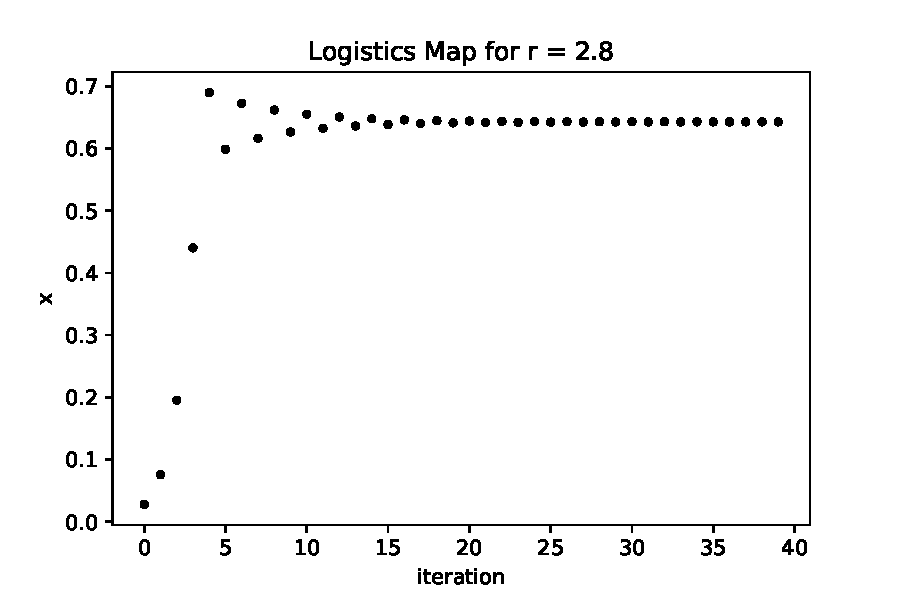
\includegraphics[width=0.65\textwidth]{figs/plotting/converge.pdf} 
\caption{Convergence of the logistic map for $r=2.8$}
\label{fig:logmapconv}
\end{center}
\end{figure}

\plot Plot the time evolution of the logistics map for $r=2.8$ for 40
iterations, starting from $p_0=0.1$ as in Fig.~\ref{fig:logmapconv}.
To create a plot, you'll need an array containing the $p$ values
(these correspond to the $y$ axis in the plot) which you can construct
as in the previous exercise.  But what about the $x$ axis values?
Since your array of $p$ values contains $[p_0, p_1, p_2 \ldots p_n]$
the corresponding array of indices is simply $[0,1,2 \ldots 3]$ which
you can construct using \pyth{np.arrange}.\\

Your results from the previous exercise should reproduce
Fig.~\ref{fig:logmapconv}.  This shows that for $r=2.8$ the logistics
map converges to a value of about 0.64.  But this non-linear recursion
relationship does not always converge to a single value.\\

\plot Plot the time evolution of the logistics map for $r=3.2$ for 40
iterations, starting from $p_0=0.1$.\\

Notice that now the system oscillates between two values (near 0.5 and 0.8).\\

\plot Plot the time evolution of the logistics map for $r=3.5$ for 40
iterations, starting from $p_0=0.1$.\\

\begin{figure}[htbp]
\begin{center}
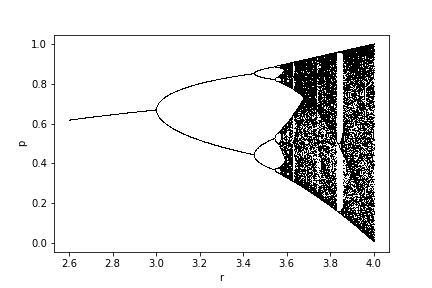
\includegraphics[width=0.65\textwidth]{figs/plotting/logmap.png} 
\caption{Long-term behavior of the logistics map as a function of parameter $r$.}
\label{fig:logmap}
\end{center}
\end{figure}

Notice that now the system oscillates between four values.  This is an
example of bifurcation in the approach to chaos.  To show this more
clearly, we'd like to produce a plot as in Fig.~\ref{fig:logmap}.  For
each $r$ value, this shows the $p$ values from 100 iterations {\em
  after} the first 1000 iterations.  This shows the {\em long term
  behavior} of the logistics map.  We can clearly see that for $r=2.8$
the $p$ values converge to one single value and for $r=3.2$ there are
two values just as in the previous exercises.  These bifurcations
continue until the system becomes chaotic (oscillating between many
different values) with occassional windows of stability.

To produce this plot for yourself, start by considering this snippet:
\begin{python}
Nr = 5
r = np.linspace(2.6,4,Nr)
p = logmap(0.1,r)
print(p)
p = logmap(p,r)
print(p)
\end{python}
Here we create a numpy array of $r$ values, and pass that to our
\pyth{logmap} function instead of a single value.  The operations
within the function are applied elementwise to the array, and the
result is that instead of a single $p$ value, the call to to
\pyth{logmap(0.1,r)} returns an array of $p$ values, one for each $r$
value.  This is just what we need to make the plot in Fig.~\ref{fig:logmap}.\\

\plot Run (and understand!) the snippet and make a plot of $p$ versus
$r$.  Understand that you are plotting $p_2$ as a function $r$!  Use
the \pyth{\"k,\"} format option (black pixels) when plotting.  Comment
out the print statements and increase $Nr$ to 100.\\

\plot Make a plot that is {\em almost} like that of
Fig.~\ref{fig:logmap} by plotting $p_{1001}$ versus $r$.  Hint:
in the code above, instead of one call to \pyth{p = logmap(p, r)} use a for loop which
calls this 1000 times.\\

You should start to see features of the Fig.~\ref{fig:logmap} but you are only plotting one $p$ value for each $r$.  To see the bifurcations and chaos, you'll need to plot about 100 $p$ values at each $r$ value.\\

\plot Reproduce the plot in Fig.~\ref{fig:logmap}.  Hint: instead of plotting just $p_{1001}$ as in the previous exercise, plot the next 100 values as well.  Increase the number of $r$ values plotted to 1000.  Add appropriate labels to each axis.\\

\plot (Optional) The bifurcation diagram which you have constructed
exhibits self-similarity.  If you zoom into an appropriate region of
the diagram, you will find a diagram which looks quite similar to the
original diagram.  Produce a plot that demonstrates this
self-similiarity by zooming into a particular region.
